
\chapter{Przegląd badań na temat eksploracji danych sportowych oraz pojęcia podstawowe}
\noindent Temat eksploracji danych sportowych i wykorzystania metod z dziedziny uczenia maszynowego w sporcie rozwinął się znacząco w ostatnich latach. Świadczą o tym chociażby organizowane corocznie konferencje poświęcone szeroko rozumianej analizie sportu, takie jak MLSA (\textit{Machine Learning and Data Mining for Sports Analytics})~\cite{MLSA20} przeprowadzane co roku w innym kraju, czy \textit{MIT Sloan Sports Analytics Conference}~\cite{MITSloan}, która ma miejsce w Stanach Zjednoczonych. Konferencje te zrzeszają nie tylko naukowców i badaczy, ale też trenerów, działaczy klubów, a nawet samych zawodników.

W przeszłości prace naukowe dotyczące piłki nożnej pojawiały się rzadziej od prac traktujących o innych dyscyplinach sportowych~\cite{ml_soccer_analytics}. Wynika to z zupełnie innej natury tego sportu. Jak wspomniano w pracy~\cite{game_classification}, piłka nożna należy do sportu z kategorii terytorialnych (\english{territory games}), które zakładają kontrolę pewnego obiektu, trzymanie go z dala od przeciwnika i stopniowego przesuwania się do pozycji, która pozwoli zdobyć punkt/bramkę. Zawodnicy zarówno defensywni, jak i ofensywni zajmują ten sam obszar boiska próbując jednocześnie uniemożliwić zdobycie punktów przez przeciwnika. Taki styl gry różni się nieco od np. baseballu, który należy do kategorii określonej jako \textit{Striking/Fielding} i charakteryzuje się zdobywaniem punktu poprzez wykonanie rzutu i biegnięcie do wyznaczonego miejsca lub uniemożliwieniem zdobycia punktu przez przeciwnika poprzez przechwycenie tego rzutu. Mając na uwadze różnice w stylach tych dyscyplin, można zauważyć, iż łatwiej jest rozbić pojedynczy mecz w baseballu na dyskretne wydarzenia do analizy, a dynamiczna i skomplikowana struktura piłki nożnej czyni taką analizę znacznie trudniejszą.

Potrzeba dostępu do szczegółowych i wyrafinowanych analiz meczów piłki nożnej spowodowała powstanie wielu komercyjnych firm takich jak \textit{Wyscout}\footnote{\url{https://wyscout.com/}} czy \textit{StatsBomb}\footnote{\url{https://statsbomb.com/}}, które dostarczają wyszukanych analiz wideo dzielących każde mecze na czynniki pierwsze przy pomocy technik rozpoznawania obrazów (\english{computer vision}) i uwzględniają niewidoczne lub trudne do wychwycenia dla ludzkiego oka szczegóły - dokładną pozycję bramkarza w momencie utraty bramki, siłę strzału, pozycję zawodnika, od którego rozpoczęła się akcja bramkowa itd.

Pomimo że techniki uczenia maszynowego w sporcie (a w szczególności w piłce nożnej) są najczęściej wykorzystywane w celu przewidywania zwycięzcy spotkania (chociażby prace z ostatniego dużego turnieju europejskiego - Euro 2016~\cite{Euro2016-1} \cite{Euro2016-2} \cite{Euro2016-3}), wiele badań dotyczy także innych zagadnień. Podejmowane są przykładowo tematy oceny umiejętności danego zawodnika (oraz jego szans na dalszy rozwój) i całej drużyny~\cite{ml_soccer_analytics} \cite{soccer_players_skill}, które mogą potencjalnie wspomóc łowców talentów szukających nowych zawodników do drużyn, czy też automatycznego wykrywania ludzkiej aktywności ruchowej~\cite{activity_recignition}, które może umożliwić na przykład znalezienie optymalnych pozycji zawodników do wykonywania strzału, podania czy sprintu.

Zrealizowanie celu tej pracy, który zakłada zbudowanie systemu przewidującego wyniki meczów piłkarskich z ligi angielskiej, wymaga dostępu do dużej ilości danych znajdujących się w wielu repozytoriach. Z uwagi na wspomnianą popularność tej dyscypliny oraz zainteresowanie nią analityków, dostęp do tych danych nie stanowi problemu, gdyż dostępnych jest wiele publicznych repozytoriów, z których te dane można pozyskać.

~

Po dokonanym przeglądzie prac o podobnej tematyce zauważono pewne interesujące zjawisko. W dużej liczbie prac~\cite{WorldCup-2018}~\cite{EloRating-1}~\cite{Euro2016-1}~\cite{Euro2016-2}~\cite{Euro2016-3} wspominany był ten sam atrybut nazywany \emph{EloRating~\footnote{\url{http://clubelo.com/}}}. Jest on  miarą przedstawiającą siłę danej drużyny obliczany na podstawie jej wyników z przeszłości. W jednej z tych prac~\cite{EloRating-1} pokazano, że wytrenowany model przy użyciu tylko jednego atrybutu (będącego różnicą wartości \emph{Elo} dla obu drużyn w dniu rozgrywania meczu) przewyższał nawet te modele, które korzystały z około 100 różnych bardziej podstawowych atrybutów. Ustępował tylko tym modelom, które jako atrybuty używały rynkowych kursów bukmacherskich. Pokazuje to, jak potencjalnie dużą wartość podczas predykcji wyniku może mieć wartość \emph{EloRating} (podobnie zresztą jak kursy proponowane przez zakłady bukmacherskie).

Na podstawie wyników i wniosków z przytoczonych artykułów, w pracy tej, podczas trenowania modeli, zdecydowano się wykorzystać zarówno atrybut \emph{EloRating} jak i rynkowe kursy bukmacherskie ze względu na ich udowodnioną skuteczność podczas predykcji. Metody na pozyskiwanie tych atrybutów zostaną szczegółowo przedstawione w rozdziale \ref{data_aggregation}.

Przegląd prac nie tylko posłużył do wstępnej selekcji możliwych do wykorzystania w algorytmie cech, ale także stanowił podstawę inspiracji do wyboru algorytmów wykorzystanych w niniejszej pracy. 

Najczęściej przejawiającym się algorytmem w analizowanych artykułach naukowych był Losowy Las drzew, tj. Random Forest \cite{CanMLPrecict} \cite{KagglePredict} \cite{BundesligaPredict} \cite{TowardDataPredict}, co ukierunkowało naturalny wybór przetestowania tego algorytmu w opisywanej pracy. Warto wspomnieć, że charakteryzował się także wysokimi wynikami predykcji w stosunku do innych algorytmów opisywanych w tych pracach. Dalszy wybór algorytmów do testowania wskazał na algorytm regresji logistycznej i algorytm metody wektorów wspierających (czyli SVM), które także w analizowanych pracach badawczych \cite{CanMLPrecict} \cite{KagglePredict} prowadziły do  obiecujących wyników. Standardowe implementacje powyższych algorytmów dostępne są w wielu popularnych bibliotekach. Jednak, w celu nie ograniczania się jedynie do metod zaimplementowanych w gotowej do użycia bibliotece \textit{scikit-learn} rozszerzono obszar zainteresowania o własną specjalnie zaimplementowaną sieć neuronową \cite{CanMLPrecict} \cite{BundesligaPredict} w oparciu o wykorzystanie modułów z biblioteki \textit{TensorFlow}. 

Ponadto z uwagi na niezbalansowanie rozkładu wyników meczów w klasach, zainteresowano się możliwością wykorzystania specjalizowanych uogólnień klasyfikatorów lub metod tzw. prze-losowanie w trakcie przetwarzania wstępnego.

Wykorzystane algorytmy szczegółowo zostaną przedstawione w rozdziale 3.3.

\section{Bazy danych i API}
Podstawą uczenia maszynowego są dane na których algorytmy mogą się uczyć, dlatego jednym z postawionych problemów było miejsce przechowywania danych jak i sposób ich pobierania.

Relacyjne bazy danych (\english{Relational databases, RBD}), których postulaty pojawiły się po raz pierwszy w artykule Edwarda Franka Codd'a \cite{Codd}, są podstawą dla wielu systemów informatycznych, mimo zwiększającej się popularności innych metod przechowywania danych, takich jak NoSQL \cite{RBD_popularity_2016}. Również w obszarze uczenia maszynowego można zauważyć dominującą popularność systemów relacyjnych baz danych. Według ankiety przeprowadzonej przez \textit{Kaggle.com}, trzy najczęściej wybierane bazy danych to relacyjne bazy danych, takie jak \textit{Microsoft SQL Server} \cite{RDB_popularity_kaggle_2020}.

RBD jest zbiorem tabel, z których każda ma za zadanie reprezentować różne encje (\english{entity}), przedstawiające część rzeczywistości. W tabelach występują rzędy oraz kolumny. Rzędy to instancje, które przedstawiają konkretne wystąpienie danej encji, a kolumny to ich atrybuty, które reprezentują cechy opisywanej części rzeczywistości. 

\begin{figure}[h] 
        \centering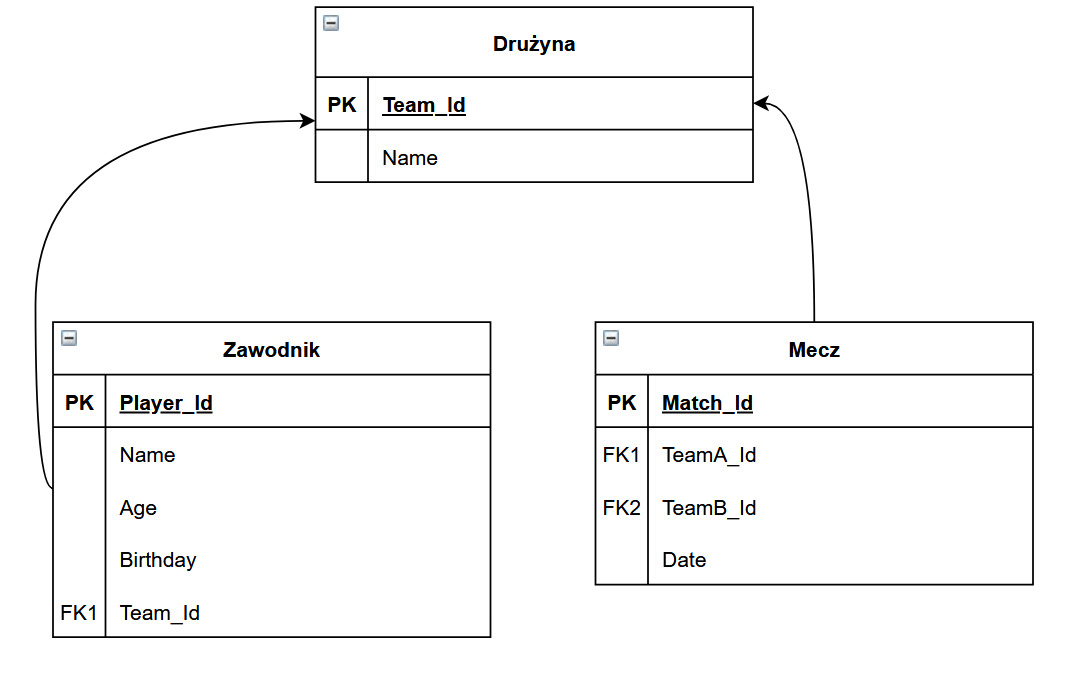
\includegraphics[width=14cm,height=10cm]{figures/Example_entities.PNG}
        \caption{Przykładowy schemat relacji encji relacyjnej bazy danych.}\label{example-Entity}
\end{figure}

Powodem dla którego nazywa się to relacyjną bazą danych jest możliwość wstawienia odnośnika jako kolumne, który wskazuje na rząd w innej tabeli. Patrząc na przykładowy schemat \ref{example-Entity}, można zauważyć, że kolumny \textit{TeamA\_Id} oraz \textit{TeamB\_Id} z tabeli \textit{Mecz}, odnoszą się do wartości w tabeli \textit{Drużyna}. Wartości w kolumnach, odwołujące się do innych tabel nazywamy \textit{kluczami obcymi}. \cite{Relational_Databases_Milan}

Obecnie istnieje duża ilość oprogramowania, umożliwiającego zarządzanie takimi bazami danych, np. \textit{Microsoft SQL Server} czy \textit{PostgreSql}, lecz wszystkie sprowadzają się do ujednoliconego standardu ISO \cite{SQL_ISO}. Zdefiniowane są tam zasady, jaką RBD powinny mieć strukturę oraz jakie typy danych zawierają. W pracy zostały użyte ze względu na łatwość dostępu do narzędzi oraz możliwości utworzenia instancji na chmurze, korzystając z Azure Cloud.

~

Problem pobierania danych dla algorytmów uczenia maszynowego został rozwiązany poprzez użycie WebAPI (\english{Web Application Programming Interfaces}). API to zbór funkcji i reguł wewnątrz aplikacji, umożliwiający interakcje z tą aplikacją za pośrednictwem oprogramowania \cite{webAPI_Mozzila}. W przypadku WebAPI korzystanie z interfejsu sprowadza się do wykonywania żądań http pod odpowiedni adres internetowy. Przykładowo, API Twitter umożliwia pobranie ostatnich wpisów podanego użytkownika, za pomocą żądania http pod udostępniony URL (\english{Uniform Resource Locator}) oraz wiele innych interakcji z stroną \cite{Twitter_API}.

Użycie WebAPI jako sposobu udostępniania danych umożliwia nam wstępnie zagregowanie danych do ujednoliconego formatu JSON (\english{JavaScript Object Notation}), dla którego istnieje wiele parserów, dzięki czemu można z nim łatwo pracować \cite{JsonParserPython}.

\section{Wstępne przetwarzanie i wizualizacja danych}

\noindent 

Jednym z kluczowych aspektów mocno wpływających na powodzenie każdego projektu związanego z uczeniem maszynowym jest stworzenie odpowiedniego zbioru cech (\english{features}) na podstawie poprawnie przygotowanych danych. W kontekście uczenia maszynowego, cecha to indywidualna, mierzalna własność lub charakterystyka pewnego obserwowanego zjawiska~\cite{Wiki:Feature}. W przypadku modelu przewidującego wyniki meczów piłkarskich, przykładem cechy może być liczba żółtych kartek uzyskanych przez drużynę gospodarzy w ostatnim meczu lub średni procent posiadania piłki drużyny gości w meczach obecnego sezonu.

Metody konstruowania zbioru danych są często automatyzowane lecz wtedy  pozbawione ścisłej kontroli, stąd mogą one zawierać różnego rodzaju błędy, takie jak wartości spoza zakresu (np. wiek: -20), nierealistyczne kombinacje wartości (płeć: mężczyzna, w ciąży: tak) lub pominięte atrybuty dla niektórych rekordów. Ważne jest, aby takie błędy wychwycić już na etapie wstępnego przetwarzania i nie dopuścić ich do danych wejściowych dla algorytmów uczących się. Pomocna może się tutaj okazać wizualizacja dokonana w celu tzw. eksploracyjnej analizie danych. Przykładowo dla atrybutów można wizualizować rozkład ich wartości przy pomocy histogramów lub wypisywać ich podstawowe statystyki (m.in. średnie, mediany, wartości minimalne, maksymalne) w celu weryfikacji poprawności ich zakresów i typów.

W ogólności można oczekiwać, że system będzie w stanie nauczyć się przewidywać wyniki tylko mając do dyspozycji jak najwięcej znaczących cech i jak najmniej tych mało znaczących. Zgodnie z popularnym angielskim zwrotem w obszarze przetwarzania informacji i analizie danych -  \definicja{śmieci na wejściu – śmieci na wyjściu} (\english{Garbage In, Garbage Out, GIGO}), nawet skuteczny i poprawnie działający program w przypadku otrzymania na wejściu błędnych danych, da na wyjściu niepoprawne oraz mało użyteczne wyniki, stąd tak ważne jest uprzednie przygotowanie danych.

Wstępne przetwarzanie (\english{preprocessing}) w projektowanym systemie składa się z jednorazowego dokonania wizualizacji posiadanych danych (która będzie szczegółowo przedstawiona w późniejszym rozdziale) w celu pogłębienia wiedzy na ich temat i wyszukania potencjalnych braków lub błędów. Następnym zadaniem, wykonywanym każdorazowo przy tworzeniu zbioru danych, którego przeznaczeniem jest użycie podczas testowania różnego rodzaju algorytmów, jest pobranie interesujących danych z bazy, przetworzenie ich, czyli poradzenie sobie z m.in. wartościami pustymi i stworzenie na ich podstawie wektora cech dla każdego rekordu (w przypadku naszego systemu jest to pojedynczy mecz). \textbf{Częstymi metodami na ...???}  

Wynikiem etapu wstępnego przetwarzania jest tzw. zbiór treningowy (\english{training set}), który zostanie omówiony w podrozdziale traktującym o algorytmach uczenia maszynowego.

\section{Algorytmy uczenia maszynowego}
Uczeniem maszynowym nazywa się grupę metod informatyki umożliwiające automatycznie \textbf{uczenie się z danych / przykładów historycznych} tak aby działać lepiej na nowych a podobnych przykładach \cite{Geron}. %Nieodłącznym elementami związanymi z tą dziedziną są takie pojęcia jak:

Uczenie tego rodzaju wymaga przetwarzania dwóch rodzajów danych:

\begin{itemize}
    \item zbiór treningowy (\english{training set}) - zbiór uczący zawierający dane używane do trenowania stworzonego przez nas sytemu (algorytmu uczącego się)
    \item zbiór testowy (\english{test set}) - zbiór zawierający część danych, na których dokonywana jest predykcja odpowiednich wartości przez skonstruowany system.
\end{itemize}
Warto podkreślić, że dane zawierające się w zbiorze testowym nie występują w zbiorze treningowym, co daje nam pewność, że algorytm nie będzie miał wcześniej do czynienia z danymi, na których ma wykonać predykcję aniżeli dopiero na etapie tejże predykcji. Wiąże się to z oceną możliwości uogólniania systemów uczących się, 

Istnieje wiele typów uczenia maszynowego, że warto podzielić je na ogólne kategorie na podstawie takich czynników, jak:
\begin{itemize}
    \item nadzór człowieka w procesie trenowania (uczenie nadzorowane, nienadzorowane, półnadzorowane i uczenie przez wzmacnianie)
    \item możliwość uczenia się w czasie rzeczywistym (uczenie przyrostowe i wsadowe)
    \item sposób pracy: proste porównywanie punktów danych (onserwacji, przykładów) ze znanymi innymi punktami lub, podobnie do naukowców, wykrywanie wzorców w danych uczących i tworzenie modelu predykcyjnego (uczenie z przykładów i uczenie z modelu)
\end{itemize}

Konstruowany system do predykcji wyniku meczu piłkarskiego jest przykładem systemu wykorzystującego uczenie nadzorowane. W uczeniu nadzorowanym (\english{supervised learning}) dane uczące przekazywane algorytmowi (wektor cech nt. danego meczu) zawierają dołączone rozwiązania problemu, tzw. etykiety (\english{labels}) (wynik danego meczu). \cite{Geron}

\begin{figure}[h] 
        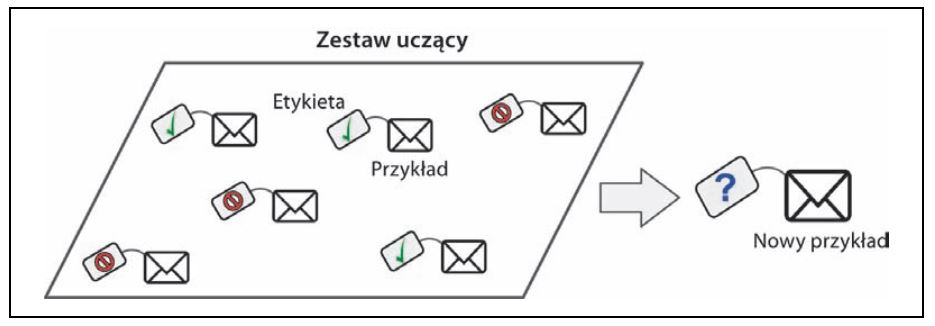
\includegraphics[width=15cm]{figures/supervised-learning.JPG}
        \caption{Zbiór danych uczących zaopatrzony w etykiety, stosowany w uczeniu nadzorowanym}
\end{figure}

\newpage

\subsection{Regresja Logistyczna}
\definicja{Regresja logistyczna} (\english{Logistic Regression}) - jedna z powszechnie używanych metod klasyfikacji. Klasyfikacja ta może być użyta, gdy przykład przypisywany jest do jednej z dwóch klas (klasyfikacja binarna) \cite{PPlonski}. Istnieją także rozszerzone modele regresji logistycznej obsługujące możliwą predykcję do więcej niż dwóch klas (klasyfikacja wieloklasowa). Regresja logistyczna oparta jest o specyficzny system prawdopodobieństw i funkcji sigmoidalnej, na podstawie której wyznaczana jest przynależność danej obserwacji do odpowiedniej klasy.\\

Prawdopodobieństwo wynikowe przynależności danej obserwacji do podanej klasy możemy wyrazić za pomocą następującego wzoru:
\begin{equation}
    P(Y|x) = \frac{\exp^{(az + b)}}{1 + \exp^{(az + b)}}
\end{equation}

gdzie:
\begin{itemize}
    \item z - zmienna niezależna (\textit{i-ta})
    \item a - współczynnik regresji logistycznej dla \textit{i-tej} zmiennej niezależnej
    \item b - stała regresji zapewniająca przesunięcie hiperpłaszczyzny decyzyjnej klasyfikatora w przestrzeni wag
\end{itemize}


Wyrażenie $\exp^{(az + b)}$ określono jako szansę i jest to stosunek prawdopodobieństwa sukcesu do prawdopodobieństwa porażki. Klasyczne prawdopodobieństwo wyrażone jako stosunek liczby sukcesów do liczby wszystkich prób przyjmuje wartości z zakresu (0;1), natomiast szansa ma tę zaletę, że przyjmuje wartości z zakresu $(0;\infty)$, co przekłada się na fakt, że logarytm szansy przyjmuje wartości z zakresu $(-\infty;\infty)$ \cite{Hosmer}. Funkcję przekształcająca prawdopodobieństwo na logarytm szansy nazywana jest funkcją sigmoidalną, która opisana jest następującym wzorem:\\

\begin{equation}
    f(z) = \frac{1}{1 + \exp^{-(az + b)}}
\end{equation}


\begin{figure}[h] 
        \centering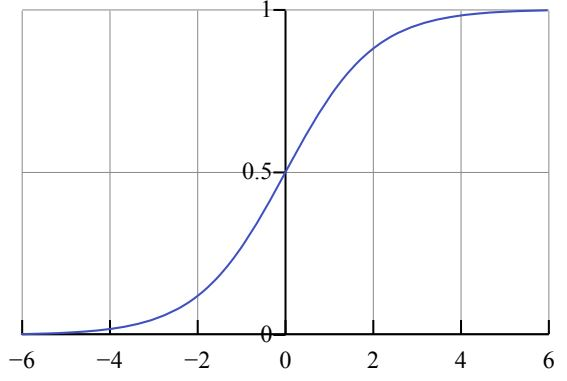
\includegraphics[width=15cm]{figures/sigmoidFunc.JPG}
        \caption{Krzywa regresji logistycznej - funkcja sigmoidalna \cite{MGrzyb}}
\end{figure}

\newpage
Z powyższego wzoru można zauważyć, że funkcja sigmoidalna daje wynik ciągły, który następnie sprowadzany jest do wyniku binarnego:

\[
y = 
    \begin{cases}
            0,& f(z) < 0.5\\
            1,& f(z) \ge 0.5
    \end{cases}
\]

\newpage
\subsection{Las losowy}
\definicja{Las losowy} (\english{Random Forest}) - zbiór klasyfikatorów (\english{ensemble classifier}), w którym każdy pojedynczy klasyfikator jest drzewem decyzyjnym uczonym bez zatrzymywania - pruningu \cite{PPlonski}. W celu zrozumienia zasady lasu losowego trzeba najpierw zrozumieć ideę drzewa decyzyjnego. Drzewa decyzyjne (\english{decision trees}) opierają się o drzewiastą strukturę. Proces klasyfikacyjny budowany jest w sposób iteracyjny począwszy od korzenia aż do liści. W kolejnych iteracjach dodawane są węzły składające się z odpowiednio dobranych atrybutów. Atrybuty są wybierane przez tzw. miary oceny atrybutów, w kolejności mającej zmaksymalizować zysk informacyjny z danego węzła (najczęściej wykorzystujący entropię informacji). Do najpopularniejszymi algorytmów wyboru cech można zaliczyć takie algorytmy jak \cite{DrzewoAlg}:
\begin{itemize}
    \item Algorytm CART (\english{Classification and Regression Tree}) - w algorytmie tym wykorzystano tzw indeks Gini'ego (\english{Gini's index}) oraz specyficzną metodę redukcji rozmiarów - pruning
    \item Algorytm C4.5 - w algorytmie tym wykorzystano wzasadył podziału opartych na entropii, m.in. reguła względnego zysku (\english{gain ratio}) zwana także współczynnikiem przyrostu informacji oraz pesymistyczne podejście do redukcji.
\end{itemize}
Cały proces ma swój koniec w momencie, gdy wszystkie przykłady uczące w liściu są przypisane do tej samej klasie lub gdy zabraknie klas do podziału. Budując pełne drzewo decyzyjne istnieje duże prawdopodobieństwo nadmiernego dopasowania algorytmu, co jest częstym problemem w przypadku podstawowej wersji drzewa decyzyjnego. \cite{MGrzyb}, dlatego rozważano metody redukcji ich rozmiarów.\\

Przykładowy model drzewa decyzyjnego:
\begin{figure}[h] 
        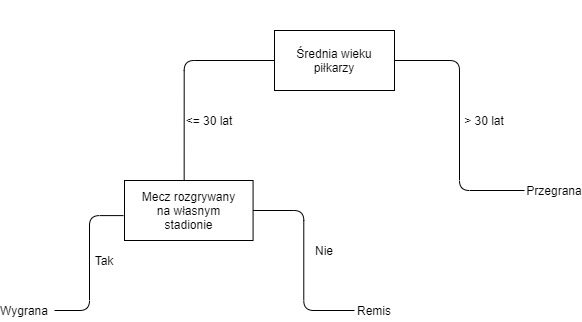
\includegraphics[width=14cm]{figures/decTree.jpg}
        \caption{Przykładowy model drzewa decyzyjnego}
\end{figure}

Na podstawie powyższego modelu zostanie przeprowadzone proste wnioskowanie decyzyjne. Zostało założone, że obserwacja wyróżnia się następującymi atrybutami:
\begin{itemize}
    \item Średnia wieku piłkarzy - 25.4 lat
    \item Mecz rozgrywany na własnym stadionie - Nie
\end{itemize}
Wartości wszystkich potrzebnych do wnioskowania atrybutów są znane, wobec czego proces predykcji jest w stanie się rozpocząć zaczynając wnioskowanie od korzenia. Średnia wieku piłkarzy jest mniejsza niż 30 lat, wobec czego proces kieruje się do lewej gałęzi drzewa. Kolejno sprawdzony zostaje fakt czy badany przez nas mecz jest rozgrywany na własnym stadionie - według badanej obserwacji mecz jest rozgrywany na wyjeździe w związku z czym odpowiedź jest przecząca i proces kieruje się prawą gałęzią drzewa. W tym momencie proces dochodzi do liścia z etykietą ,,Remis'', która to etykieta jest ostateczną predykcją wyniku meczu na podstawie wnioskowania w tym drzewie decyzyjnym.\\

Po przedstawieniu zasad konstruowania drzewa decyzyjnego omówiony zostanie algorytm lasu losowego, który tak jak zostało wspomniane jest zbiorem klasyfikatorów, gdzie każdy klasyfikator jest drzewem decyzyjnym. Każde drzewo wchodzące w skład lasu losowego jest uczone na specjalnie wylosowanej dla niego próbce danych pochodzącej ze zbioru uczącego, treningowego (tzw. losowanie bootstrapowe). Dodatkowo, w trakcie budowania drzewa decyzyjnego nie wszystkie atrybuty są brane pod uwagę przy wyznaczaniu testu na atrybucie do podziału w węźle. Losowany jest pewien podzbiór atrybutów, na podstawie których wyznaczany jest najlepszy podział na atrybucie w węźle. Obie opisane techniki działania na próbce danych i pewnym wylosowanym podzbiorze atrybutów stosowane są w celu zwiększenia stabilności odpowiedzi algorytmu i jego ochrony przed nadmiernym dopasowaniem do danych uczących, co było jedną z największych wad pojedynczego drzewa decyzyjnego i co przekłada się dodatkowo na lepszą skuteczność działania klasyfikatora na nowych danych. W trakcie przewidywania klasy dla próbki jest ona pokazywana wszystkim drzewom decyzyjnym, a jako końcowa decyzja o przynależności do klasy traktowanej jest przypisanie do klasy najczęściej wskazywanej przez drzewa decyzyjne w lesie. Dodatkowym plusem lasu losowego jest umiejętność wyznaczenia ważności atrybutów wejściowych. \cite{PPlonski}\\

Przykładowy proces wnioskowania na podstawie algorytmu lasu losowego można zobaczyć na poniższym rysunku
\begin{figure}[h] 
        \centering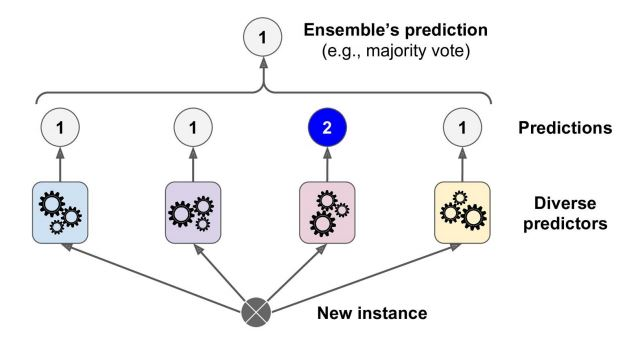
\includegraphics[width=14cm]{figures/randomForestModel.JPG}
        \caption{Przykładowy model lasu losowego \cite{Geron}}
\end{figure}

\newpage

\subsection{Metoda Wektorów Wspierających - SVM}
\definicja{Metoda wektorów wspierających - nośnych} (\english{Support Vector Machine, SVM}), jest to nadzorowana technika uczenia maszynowego wykorzystywana do zadań klasyfikacji oraz regresji. Technika ta została opracowana w laboratorium AT\&T Bell poprzez Vladimira Naumovicha Vapnika wraz ze współpracownikami (Boser i in., 1992, Guyon i in., 1993, Vapnik i in., 1997). \cite{Wiki:SVM}. Głównym założeniem tej metody jest wyznaczenie hiperpłaszczyzny, która ma za zadanie rozdzielić przy pomocy maksymalnego marginesu przykłady należące do różnych klas. W przypadku występowania więcej niż dwóch klas, metoda ta wykorzystuję technikę \definicja{OvR} (\english{One-vs-Rest}), która polega na szkoleniu jednego klasyfikatora na klasę, z próbkami z tej klasy jako pozytywne próbki, a inne próbki jako negatywy. Formalnie problem klasyfikacji przedstawia się następująco \cite{Prezentacja:SVM2}: 
\begin{itemize}
    \item W przestrzeni danych (ang. measurement space) $\omega$ znajdują się wektory danych x stanowiące próbkę uczącą D, należące do dwóch klas\\
    \begin{equation}
D = \big\{(x_{i}, c_{i}) | x_{i} \in R^{p}, c_{i} \in \{-1, 1\}\big\}_{i=1}^{N}
    \end{equation}
    \item Szukany jest klasyfikator pozwalający na podział całej przestrzeni $\omega$ na dwa rozłączne obszary odpowiadającej klasom {1,-1} oraz pozwalający jak najlepiej klasyfikować nowe obiekty x do klas
    \item Podejście opiera się na znalezieniu tzw. granicy decyzyjnej między klasami → g( x )
\end{itemize}
Dodatkowo dwie klasy są liniowo separowalne, jeśli istnieje hiperpłaszczyzna H postaci: \[g(x) = w^Tx + b\] przyjmująca wartości: 

\[
    \begin{cases}
            g(x_{i}) > 0,& x_{i} \in 1 \\
            g(x_{i}) < 0,& x_{i} \in -1
    \end{cases}
\]
\\

Linia granicy decyzyjnej nie tylko oddziela dwie klasy, ale także pozostaje jak najdalej od najbliższych instancji. Jak pokazano na rysunku \ref{SVM-margines} problemem poza znalezieniem $B_{2}$ jest również znalezienie szerokości wspomnianej granicy. Niestety nie ma na to idealnego rozwiązania i konieczne jest wybranie cech, które są bardziej odpowiednie dla naszego problemu. Szerszy margines to lepsze własności generalizacji, mniejsza podatność na
ewentualne przeuczenie (\english{overfitting}), a z kolei wykorzystanie wąskiego marginesu skutkuje radykalną zmianą klasyfikacji przy małej zmianie granicy. Jednak ze względu na oszacowanie górnej granicy błędu ze względu na błąd uczący częściej wybiera się jak najszerszy margines w celu lepszego uogólniania w bardziej skomplikowanych modelach.

\begin{figure}[H] 
        \centering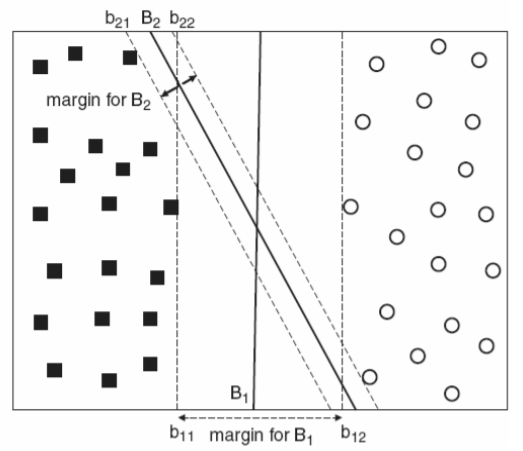
\includegraphics[width=6cm,height=6cm]{figures/SVM-margin.png}
        \caption{Margines granicy decyzyjnej}\label{SVM-margines}
\end{figure}
Konsekwentnie, problem maszyn wektorów nośnych sprowadza się do poszukiwania maksymalnego marginesu klasyfikacji: $w x + b = 0$ gdzie \definicja{w} oraz \definicja{b} są parametrami modelu.
\[
y = 
    \begin{cases}
            1,&  wx+b > 0\\
            -1,& wx+b < 0
    \end{cases}
\]
Dodatkowo parametry granicy wyznacza się tak, aby maksymalne marginesy (margines to odległość między \definicja{bi1} oraz \definicja{bi2}) \definicja{bi1} i \definicja{bi2} były miejscem geometrycznym punktów \definicja{x} spełniających warunki \ref{SVM-marginesEq}:
\[
    \begin{cases}
            bi1,&  wx+b = 1\\
            bi2,& wx+b= -1
    \end{cases}
\]
\begin{figure}[H] 
        \centering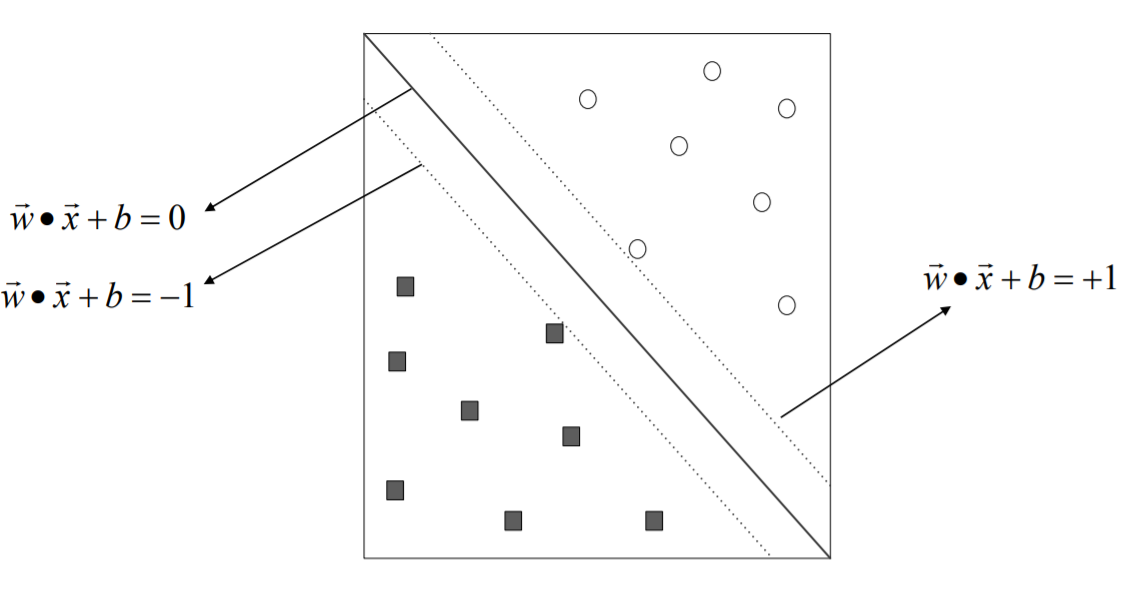
\includegraphics[width=14cm,height=6cm]{figures/SVM-marginEq.png}
        \caption{Wyznaczanie marginesu granicy decyzyjnej}\label{SVM-marginesEq}
\end{figure}

Tak więc problem ten sprowadza się do optymalizacji kwadratowej z liniowymi ograniczeniami (uogólnione zadanie optymalizacji). 
Czasami jednak zdarza się sytuacja podczas której nie ma możliwości w pełni liniowej separacji klas. W takiej sytuacji wykorzystuje się zmienne osłabiające \definicja{$\xi_{i} \ge 0$}, które dobiera się dla każdego przykładu uczącego. Jej wartość zmniejsza margines separacji. Jeżeli $0 \le \xi_{i} \le 1$, to punkt danych $(xi,di)$ leży wewnątrz strefy separacji, ale po właściwej stronie, a w sytuacji gdy $\xi_{i} \ge 1$, to punkt leży po niewłaściwej stronie hiperpłaszczyzny i nastąpi błąd klasyfikacji. 
\[
    \begin{cases}
            bi1,&  wx+b = 1 - \xi\\
            bi2,& wx+b= -1 + \xi
    \end{cases}
\]
Również tutaj występuje konflikt doboru marginesu. Szeroki margines to dużo błędów i odwrotnie. Kończąc rozważania dotyczące liniowej maszyny wektorów nośnych, obecny problem znalezienia granicy decyzyjnej sprowadza się do minimalizacji wyrażenia:
\[
L(w) = \frac{\|\vec{w}\|}{2} + C\big(\sum_{i=1}^{N}\xi_{i}^{k}\big)
\]
z ograniczeniami:
\[
f(\vec{x_{i}}) = 
    \begin{cases}
            1 &  \text{if}\ \vec{w} \bullet \vec{x_{i}}+b \ge 1 - \xi_{i}\\
            -1 &  \text{if}\ \vec{w} \bullet \vec{x_{i}}+b \le 1 + \xi_{i}
    \end{cases}
\]
gdzie parametr \definicja{C} to ocena straty związanej z każdym błędnie klasyfikowanym punktem dla którego $\xi > 0$. Problem ten to problem dualny i istnieją techniki pozwalające na jego rozwiązanie.

Dodatkowym problemem w tej metodzie jest fakt, że najczęściej klasy nie są liniowo separowane. Jednym ze sposobów na poradzenie sobie z tym problemem jest transformowanie, projekcja danych wejściowych do przestrzeni o większej liczbie wymiarów, w której dane, z dużym prawdopodobieństwem będą separowane liniowo. Funkcja decyzyjna po przekształceniu ma się następująco:
\[
g(x) = w\varphi(x) + b
\]
Problem ten jest trudny obliczeniowo do wykonania, lecz można sobie z nim poradzić za pomocą kerneli, funkcji jądrowych. Funkcje te wywodzą się z badań liniowych przestrzeni wektorowych, przestrzeni Hilberta, Banacha. Dzięki nim można wyznaczyć potrzebne parametry do rozwiązania naszego problemu. Najczęściej stosowane jądra w metodzie maszyn wektorów nośnych to: Gaussowskie, wielomianowe i sigmoidalne. Dzięki nim, nie musimy znać funkcji transformacji, a jedynie funkcję kernela co pozwala nam na pracę w nowej przestrzeni. 

Można zauważyć, że metoda SVM jest silną metodą pozwalającą na rozwiązywanie problemów klasyfikacji w wielowymiarowej przestrzeni danych. Dzięki niej można skutecznie uogólniać nowe przykłady i przydzielać im odpowiednie klasy zdefiniowane dla konkretnego problemu.

\newpage

\subsection{Sztuczne Sieci Neuronowe - SNN}
\label{SNN-opis}

\definicja{Sztuczna sieć neuronowa} ogólna nazwa struktur matematycznych i ich programowych lub sprzętowych modeli, realizujących obliczenia lub przetwarzanie sygnałów poprzez rzędy elementów przetwarzających, zwanych sztucznymi neuronami, wykonujących pewną podstawową operację na swoim wejściu. Oryginalną inspiracją takiej struktury była budowa naturalnych neuronów, łączących je synaps, oraz układów nerwowych, w szczególności mózgu \cite{Wiki:SNN}. Sztuczne sieci neuronowe charakteryzują się tym, że mają zdolność do odwzorowania różnych zależności pomiędzy sygnałami wejściowymi i wyjściowymi. Sztuczna sieć neuronowa składa się z wielu połączonych neuronów, a kady neuron można interpretować jako pewna kombinacja matematyczna cech wejściowych wraz z przypisanymi im wagami. Wyjście neuronu to pewna funkcja matematyczna, która przekształca daną kombinację danych wejściowych i przekazuje taki wynik na swoje wyjście. Graficzna reprezentacja takiego neuronu ma się następująco \cite{Prezentacja:SNN,KrawiecStefanowski03}:
\begin{figure}[H] 
        \centering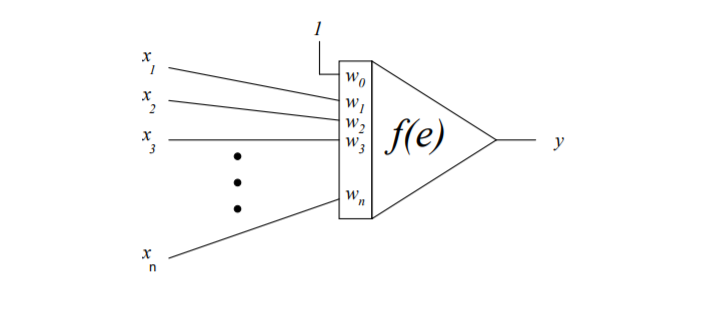
\includegraphics[width=12cm,height=6cm]{figures/SNN.png}
        \caption{Sztuczny neuron}\label{SVM-neuron}
\end{figure}

Podstawowe elementy składowe neuronu: 
\begin{itemize}
    \item n wejść neuronu wraz z wagami $w_{i}$ (wektor wag w i wektor sygnałów wejściowych x)
    \item jeden sygnał wyjściowy y
    \item pobudzenie e neuronu jako suma ważona sygnałów wejściowych
pomniejszona o próg $\Theta$
\[
e = \sum_{i=1}^{N} w_{i} x_{i} - \Theta = w^{T} x - \Theta
\]
wprowadźmy wagę $w_{0}= \Theta$, podłączonej do stałego sygnału $x_{0} = 1$;
wówczas: 
\[
e = \sum_{i=0}^{N} w_{i} x_{i}  = w^{T} x
\]
\item funkcja aktywacji (przejścia):
\[
y = f(e)
\]
\end{itemize}
Kluczowe znaczenie dla działania neuronu ma funkcja aktywacji. Jest do wyboru funkcja liniowa lub nielinowa (ciągła i nieciągła, unipolarna i bipolarna).

W literaturze wyróżnia się dwa ogólne typy sieci neuronowych i są to: jednokierunkowe SNN oraz rekurencjne SNN (sieci ze sprzężeniami zwrotnymi np. sieć Hopfielda albo sieci uczenia się przez współzawodnictwo).
Sieci jednokierunkowe to sieci o jednym kierunku przepływu sygnałów. Szczególnym przypadkiem architektury jednokierunkowej jest sieć warstwowa, reprezentująca zdecydowanie najpopularniejszą topologię.
\begin{figure}[H] 
        \centering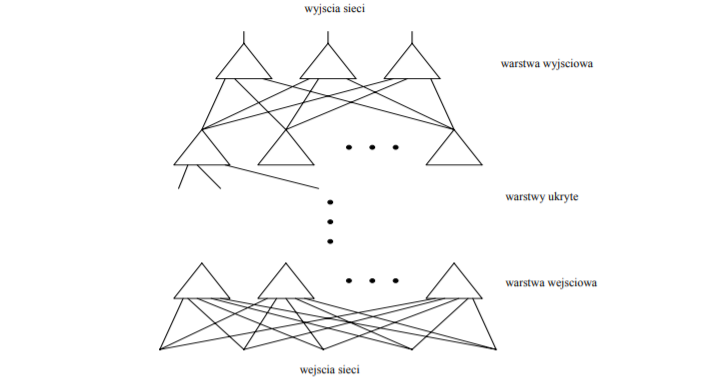
\includegraphics[width=12cm,height=6cm]{figures/ArchitekturaSNN.png}
        \caption{Sieć warstwowa jednokierunkowa}\label{SVM-neuron}
\end{figure}

Zasady łączenia neuronów między sobą:
\begin{itemize}
    \item każdy neuron z każdym,
    \item połączenia między kolejnymi warstwami w sieciach warstwowych,
    \item tylko z pewną grupą neuronów, najczęściej z tzw. sąsiedztwem
\end{itemize}

W celu uzyskania wyników wykorzystuje się \definicja{uczenie nadzorowane}. Dany jest zbiór przykładów uczących składający się z par wejście-wyjście $(x_{j}, z_{j})$, gdzie $z_{j}$ jest pożądaną odpowiedzią sieci na sygnały wejściowe $x_{j} (j=1,..m)$. Zadaniem sieci jest nauczyć się możliwie jak najdokładniej funkcji przybliżającej powiązanie wejścia z wyjściem. Odległość pomiędzy rzeczywistą a pożądaną odpowiedzią sieci jest
miarą błędu używaną do korekcji wag sieci. Typowym przykładem jest uczenie sieci wielowarstwowej algorytmem wstecznej propagacji błędu; każdy neuron lokalnie zmniejsza swój błąd stosując metodę spadku gradientu.

W celu uczenia sieci neuronowych wykorzystuje się kilka reguł i są nimi między innymi: \definicja{reguła Widrowa-Hoffa} oraz \definicja{reguła delta}. Pierwsza z nich dotyczy uczenia nadzorowanego sieci jednokierunkowych, gdzie minimalizuje się błąd pomiędzy pożądaną a aktualną odpowiedzią. 
\[
\delta^{j} = z^{j} - y^{j} = z^{j} - w^{T}x^{j}
\]

Korekta wag jest następująca \cite{Widrow}:
\begin{equation}
\label{eqn:delta}
\delta w_{i} = \eta \delta^{j} x^{j}_{i}
\end{equation}
Reguła delta z kolei obowiązuje dla neuronów z ciągłymi funkcjami aktywacji i nadzorowanego trybu uczenia. Regułę delta wyprowadza się jako wynik minimalizacji kryterium błędu średnio-kwadratowego Q.
\[
    Q = \frac{1}{2}\sum_{j=1}^{N} \big( z^{j} - y^{j}\big)^{2} = \sum_{j}^{N}Q^{j}, Q^{j} = \frac{1}{2}(\delta^{j})^{2}
\]

Korekta wag:
\[
\delta w_{i} = \eta \delta^{j} (1 - y^{j}) f'(e^{j}) x^{j}_{i}
\]
gdzie $f'()$ oznacza pochodną funkcji aktywacji. Stosowana jest do uczenia wielowarstwowych sieci neuronowych wraz z algorytmem wstecznej propagacji błędów \cite{Rumelhart}. Sieci charakterystyczne cechują się pewnymi właściwościami \cite{Mitchell}:
\begin{itemize}
    \item Przykłady uczące opisane są przez pary atrybut-wartość (na ogół
zdefiniowanych na skalach liczbowych,
    \item Przybliżana funkcja może mieć wartości dyskretne lub rzeczywiste;
może być także wektorem wartości,
 \item Dane mogą zawierać błędy lub podlegać zniekształceniu. SSN są
odporne na różnego rodzaju uszkodzenia danych, 
    \item Akceptowalny jest długi czas uczenia sieci,
    \item Akceptacja dla potencjalnie dużej liczby parametrów algorytmu,
które wymagają dostrojenia metodami eksperymentalnymi,
    \item Zadanie nie wymaga rozumienia przez człowieka funkcji
nauczonej przez SNN - trudności z interpretacją wiedzy nabytej
przez sieć (rozwijający się w tym momencie sektor uczenia maszynowego XAI - \english{explainable artificial intelligence}).
\end{itemize}

Jednak kluczowym konceptem sprawiającym, że sztuczne sieci neuronowe są tak popularne i oferujące wiele możliwości jest wsteczna propagacja błędów, czyli sposób w jaki sieć nabywa umiejętności generalizowania danych i przyporządkowywania odpowiednich wartości. Błąd k-tego neuronu w l-tej warstwie jest równy sumie błędów popełnionych przez neurony (p) z warstwy l+1-szej ważonych po wagach $w_{k(p,l+1)}$ łączących ten neuron z neuronami tej warstwy \cite{Prezentacja:SNN}: 

\[
\delta_{(k,l)}^{j} = \sum_{p=1}^{N_{l+1}} W^{j}_{k(p, l+1)} \delta_{(p,l+1)}^{j}
\]

Na podstawie wstecznej propagacji błędów, sieci neuronowe modyfikują wagi dla każdego neuronu dopowiadające danym wejściowym w celu minimalizacji funkcji nazywanej \definicja{funkcją straty}.

Wartości początkowe wag muszą być zainicjowane przed przystąpieniem do procesu uczenia i zazwyczaj dokonuje się tego w sposób losowy lub na podstawie pewnego rozkładu prawdopodobieństwa. Kluczowym czynnikiem do prędkości oraz jakości otrzymywanych wyników jest współczynnik $\eta$, który można było zauważyć w równaniu \ref{eqn:delta}. Decyduje on o wpływie błędu popełnianego przez neuron na korektę wartości wag. Właściwy dobór ma kluczowe znaczenie dla prędkości zbieżności algorytmu, a jego zbyt mała wartość spowalnia proces uczenia i zwiększa ryzyko
wpadnięcia w pułapkę lokalnego minimum \cite{Prezentacja:SNN}. 

W momencie gdy ludzie zaczęli interesować się tematem uczenia maszynowego oraz sieciami neuronowymi zaczęto szerzej zgłębiać temat stawiając coraz to trudniejsze wyzwania. Powstało mnóstwo różnych struktur sieci. Te bardzo głębokie składające się z kilkunastu, a nawet kilkuset warstw ukrytych oraz sieci, które przyjęły trochę inną koncepcję przetwarzania danych. Jednym z dużych zmian, jakie nastąpiły w kwestii przetwarzania obrazów, było zastosowanie konwolucyjnych sieci neurnowych (\english{convolutional neural network})\cite{CNN}. Struktura takiej sieci różni się od podstawowej koncepcji tym, że zamiast w pełni połączonych warstw neuronów, posiada ona \definicja{konwolucyjne warstwy}, które mają za zadanie znalezienie pewnych wzorców na obrazie - tych większych jak i tych mniejszych. Wiele zastosowanych filtrów skanujących obraz wraz z połączeniem warstwową łączącą (\english{pooling layer}) daje w rezultacie o wiele większą skuteczność w dziedzinie przetwarzania obrazów dzięki wydobywaniu z obrazów pewnych zależności oraz połączeń pomiędzy pikselami tworzącymi obiekt \cite{Prezentacja:KKCNN} \cite{Prezentacja:CNNintro}.
Inną koncepcją w głębokich sieciach neuronowych jest struktura zwana \definicja{Rekurencyjna sieć neuronowa}  \cite{Prezentacja:KKRNN}. Główną myślą w tej koncepcji było zastosowanie zwykłej głębokiej sieci neuronowej, lecz dodatkowo, poza zwykłymi połączeniami w przód, zastosowane zostały połączenia odwołujące się również do poprzednich warstw w strukturze sieci. Dzięki takiemu rozwiązaniu można było nauczyć sieć pewnych powtarzających się wzorców, które dzięki rekurencyjnym połączeniom były łatwiejsze do wykrycia \cite{Geron2}. Dodatkowo, aby zwiększyć ilość informacji, która zostanie zapamiętana przez daną strukturę sieci, zostały wprowadzone pewne jednostki, nazywane komórkami pamięci (\english{memory cell}), takimi jak \definicja{LSTM} \cite{LSTM} czy \definicja{GRU} \cite{GRU}. Technika ta otwarła wiele możliwości w przetwarzaniu szeregów czasowych oraz pozwoliła na rozpoczęcie pracy nad przetwarzaniem języka naturalnego.

Poza wymienionymi powyżej przykładami, które różniły się budową od w pełni połączonej sieci neuronowej, powstało wiele różnych koncepcji, które były tworzone z myślą o konkretnych zastosowaniach i nie sposób opisać w tym akapicie wszystkich pomysłów.

Niestety sieć neuronowa jest trudnym narzędziem i występuję w niej problem doboru wielkości warstw ukrytych, który do teraz jest problemem otwartym. 
Nie istnieje jednoznaczna reguła określająca optymalny rozmiar danej warstwy oraz ilości warstw w danej sieci przy danym zbiorze uczącym. Zbyt mała wielkość warstw czyni sieć niezdolną do adaptacji do
zadanego zbioru przykładów co skutkuje, że w trakcie uczenia błąd
średnio-kwadratowy utrzymuje dużą wartość. Zbyt duże warstwy z kolei mają problem z przeuczaniem (nauka konkretnych wartości danych wejściowych, a nie ogólnego konceptu, zarysu) \cite{Prezentacja:SNN}.

Od początku historii SNN do teraz powstało mnóstwo konceptów, pomysłów, sztuczek i schematów które zapewniają lepsze generalizowanie, szybsze zbieganie do minimum, które nie sposób zebrać i opisać w jednym miejscu. Wiele technik zapewniło uczenie bardzo dużych sieci neuronowych zapewniających stabilne gradienty (jednym z problemów podczas nauki SNN jest niestabilność gradientów, które zanikały wraz z postępem algorytmu lub wręcz eksplodowały do bardzo dużych wartości) \cite{gradient}. Powstało również wiele funkcji aktywacji oraz sposobów inicjalizacji początkowych wag sieci.

\section{Algorytmy dla danych niezbalansowanych}

\textit{Tutaj opisac MRBag} - myśle że to jest miejsce do uzupełnienia

\section{Sposób oceny wyników predykcji}
\label{section:ocenaWynikow}

Różne algorytmy dają wyniki w różnych formie. Niektóre wskazują tylko  konkretną klasę, do której przynależy konkretne wejście, a inne przyporządkowują przykładowi rozkład prawdopodobieństwa możliwych wyników klasyfikacji. W badanym w rozprawie zadaniu mamy do czynienia z obiema sytuacjami. 

Podczas doboru sposobu oceny algorytmów głównym celem jest dobranie takich miar tak, aby móc wzajemnie porównywać zastosowane algorytmy i na tej podstawie dobrać najlepsze podejście. Ocena jakości rozwiązań opierała się zatem na policzeniu \definicja{dokładności / trafności} (\english{accuracy}) na zbiorze testowym (w danych sportowych wynoszącym 10\% całego zbioru danych), macierzy pomyłek oraz wynikające z niej miary takie jak: \definicja{precyzja} (\english{precision}, interpretować ją można jako stosunek tp / (tp + fp), gdzie tp to liczba poprawnie sklasyfikowanych przykładów, a fp to liczba niepoprawnie sklasyfikowanych przykładów.), \definicja{czułość} (\english{recall}, interpretować można jako stosunek tp / (tp + fn), gdzie tp jest liczbą poprawnie sklasyfikowanych przykładów, a fn liczbą niepoprawnie sklasyfikowanych przykładów.) oraz \definicja{F-score} (\definicja{F-score} interpretuje się jako ważoną średnią harmoniczną precyzji i czułości, gdzie wynik \definicja{F-score} osiąga najwyższą wartość przy 1, a najniższą przy 0), którą wyznaczono przy użyciu średniej typu „macro” (oblicza metryki dla każdej etykiety, a następnie wyznacza ich nieważoną średnią. Metoda ta nie uwzględnia niezbalansowania danych) \cite{SKfscore}. Dodatkowo w celu porównania zastosowana została macierz pomyłek, której schemat można zobaczyć w tabeli \ref{tab:macierz}

\begin{center}
\begin{table}[H]
\renewcommand{\arraystretch}{1.5}
\caption{Macierz pomyłek dla problemu klasyfikacji}
\label{tab:macierz}
\begin{center}
\begin{tabular}{|c|c|c|c|c|}
   \cline{3-5} 
   \multicolumn{1}{c}{} & & \multicolumn{3}{c|}{Predicted} \\ \cline{3-5}
   \multicolumn{1}{c}{} & & Draw & HomeWin & AwayWin \\ \hline
   
   {Observed}
   & Draw & T & F & F \\ \cline{2-5}
   & HomeWin & F & T & F  \\ \cline{2-5}
   & AwayWin & F & F & T \\ \hline
\end{tabular}
\end{center}
\end{table}
\end{center}

W rozprawie dodatkowo przetestowano algorytmy w przyrostowy sposób, w którym dane wejściowe podzielono na bloki następujące po sobie. Następnie wyuczono algorytmy na pierwszym bloku i testowano jego działanie na koejnym bloku, który w zbiorze danych występował zaraz po bloku uczącym. Kolejno do dotychczasowego zbioru uczącego dołożono dane z poprzedniego bloku testowego i na podstawie nowego zbioru znów dokonano uczenia maszynowego by następnie dokonać ewaluacji na kolejnym fragmencie zbioru testowego. Proces ten powtarzano, aż do wykorzystania wszystkich dostępnych i przygotowanych danych.

